\documentclass[convert, margin=5mm, tikz]{standalone}
\usepackage{tikz-feynman}
\usepackage{tikz}
%\usetikzlibrary{animations}
\begin{document}
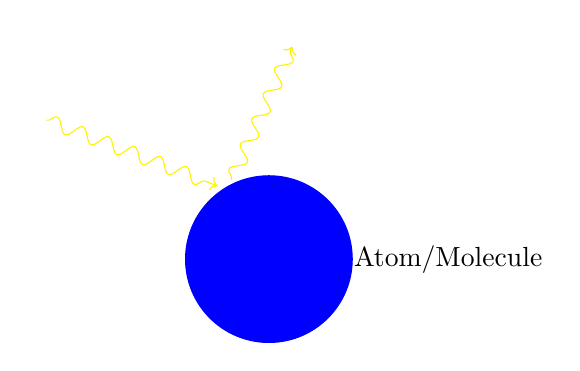
\begin{tikzpicture}
  \filldraw[fill=blue, draw=blue, outer sep = 12px] (0,0) circle (30px) node[label=right:Atom/Molecule]{};%{\small Nucleus};
  % \path[densely dotted, draw=blue] (0,0) circle (105px);
  % \filldraw[fill=blue, draw=blue] (-79px, 70px) circle (3px) node[anchor=north west]{\tiny \(e^-\)};
  \node[] (e1) at (-15px, 25px) {} ;
  \draw[->,decorate, decoration=snake, draw=yellow] (-80px, 50px) node[anchor=south east]{} -- (e1);
  \node[] (e2) at (10px, 80px) {} ;
  \draw[->,decorate, decoration=snake, draw=yellow] (e1) -- (e2);
\end{tikzpicture}
\end{document}